\documentclass[11pt,a4paper]{article}

\usepackage[margin=2.5cm]{geometry}
\usepackage{amsmath}
\usepackage{amssymb}
\usepackage{booktabs}
\usepackage{graphicx}
\usepackage[colorlinks=true,linkcolor=black,citecolor=blue,urlcolor=blue]{hyperref}

% thebibliography prints its own unnumbered "References" heading; the numbered
% \section{References} already provides it, so the next starred heading is
% swallowed once (star and title consumed together) and the sections after the
% bibliography keep the normal \section.
\makeatletter
\newcommand{\swallownextsectionstar}{%
  \let\originalsection\section
  \renewcommand{\section}{\@ifnextchar*{\swallowsectionstar}{\originalsection}}}
\def\swallowsectionstar*#1{\let\section\originalsection}
\makeatother

\title{\textbf{Parallel Dense Matrix Multiplication on Shared Memory:\\
An Empirical Study of Thread-Count Scaling}\\
\vspace{0.5cm}
\Large Big Data --- Bachelor's Degree in Data Science and Engineering (ULPGC)}

\author{\textbf{Aythami Lorenzo} \\[0.1cm]
\small University of Las Palmas de Gran Canaria \\
\small Code \& Data: \url{https://github.com/aythamilorenzo/bigdata-individual-assignments}}
\date{October 2026}

\begin{document}

\maketitle

\begin{abstract}
We study the behavior of a thread-parallel implementation of dense square
matrix multiplication used on shared memory, and compare it against its
equivalent sequential baseline: both methods are the same cache-blocked
$i$-$k$-$j$ kernel (tile side 64, float64), the parallel one distributing the
kernel's $i$-tiles across a fixed pool of $p$ worker threads. We perform an
analysis of the following elements: kernel-only runtime with warm-ups and
repeated measurements (median and interquartile range), speedup
$S(p) = T_{\mathrm{seq}} / T_p$, parallel efficiency $E(p) = S(p)/p$, the
overhead of the parallel framework measured with a single thread, and peak
resident memory, across sizes $n \in \{500, 1000, 1500, 2000\}$ and thread
counts $p \in \{1, 2, 4, 6, 8, 12, 24\}$ on a 6-core / 12-logical-processor
CPU. Our experiments provide a reproducible benchmark of one parallel
multiplication scheme across a variety of problem sizes and thread counts to
guide future research in performance analysis of data-intensive workloads.
Based on our experiments, we recommend parallel execution for the largest
tested sizes with $p$ up to the number of physical cores, and we find that
beyond that point extra threads (hyper-threaded contexts and deliberate
oversubscription) return diminishing or no additional benefit for this
kernel.
\end{abstract}

\newpage
\tableofcontents
\newpage

\section{Introduction and objective}
\label{sec:introduction}

Matrix multiplication is a canonical workload for studying how algorithms,
hardware and runtime overhead interact. Assignments 1 and 2 established the
behavior of basic and optimised \emph{sequential} implementations as $n$
grows, ending with a cache-blocked kernel as the fastest sequential method
for the largest sizes~\cite{lam1991}. This study extends that validated
kernel in the direction required by the assignment: \textbf{parallel
execution on shared memory}. A sequential baseline and a thread-parallel
implementation of the \emph{same} algorithm, numeric type, storage layout
and input matrices are compared while only the thread count varies, so the
measured effect is attributable to parallelism and not to a change of
algorithm.

\paragraph{Research question.}
\emph{RQ:} how does the thread count $p$ affect the runtime, variability,
memory, speedup and efficiency of one dense shared-memory multiplication as
$n$ grows, and when does adding threads stop helping on this machine?

\section{Background}
\label{sec:background}

The baseline kernel multiplies two $n \times n$ row-major float64 matrices
with cache blocking on the $i$-$k$-$j$ loop order: work is organised in
$64 \times 64$ tiles so that a 32~KB tile of $B$ stays resident in the
core's private cache while it is reused~\cite{lam1991,hennessy2017}. Total
arithmetic work is $2n^3$ multiply--adds.

For $p$ worker threads the natural parallel decomposition of this kernel
partitions the output rows (equivalently, the $i$-tiles) among threads:
each thread accumulates a disjoint set of rows of $C = AB$, reading $A$ and
$B$ concurrently and never writing another thread's
rows~\cite{lea2006}. With $n/p$ rows per thread the idealised model is
$T_p = T_{\mathrm{seq}}/p + T_{\mathrm{overhead}}$, giving speedup
\begin{equation}
S(p) = \frac{T_{\mathrm{seq}}(n)}{T_p(n, p)}
\end{equation}
and efficiency
\begin{equation}
E(p) = \frac{S(p)}{p} \le 1 \quad \text{(ideal case)}.
\end{equation}
Three effects keep $S(p)$ below $p$: fixed per-multiplication overheads
(task dispatch and join), memory-bandwidth and cache sharing among
cores~\cite{hennessy2017}, and hardware limits --- this CPU has 6 physical
cores with 2 hardware threads each, so $p > 6$ shares execution units and
$p > 12$ oversubscribes the hardware contexts entirely, the classical
bound of Amdahl's law once the parallel fraction meets the machine's
limits~\cite{amdahl1967,hill2008}. Superlinear
speedups, when observed, require evidence (frequency scaling, cache
residency) rather than assumption.

\section{Methodology}
\label{sec:methodology}

\subsection{Implementations}

Both methods are written in Java 17 and perform the same arithmetic on the
same storage:
\begin{itemize}
    \item \texttt{blocked\_ijk\_sequential} --- the cache-blocked kernel of
    assignment 2 (block size 64), reused and validated by its test suite;
    the mandatory \emph{equivalent baseline}. It runs on the calling thread
    and always reports $p = 1$.
    \item \texttt{blocked\_ijk\_parallel} --- the same kernel's $i$-tiles
    partitioned across a fixed pool of $p$ prestarted threads. Tile $t$ of
    $\lceil n / 64 \rceil$ belongs to thread $\lfloor t \cdot p /
    \text{tiles} \rfloor$ (contiguous ranges differing by at most one
    tile). Each worker zeroes and multiplies only its own rows, so every
    output entry has exactly one writer and accumulates over $k$ in the same
    ascending order as the sequential kernel: results are element-wise
    identical and no arithmetic locks are needed. The pool is an explicit
    fixed-size thread pool; no parallel streams, no common ForkJoin pool and
    no numerical library with internal threads are involved, so the
    reported thread count describes the actual worker configuration.
\end{itemize}
Thread creation happens outside the timed region (setup, like allocating
the output buffer); the timed region contains the per-multiplication
dispatch and join of the $p$ tasks plus the tile computation --- the
framework overhead that the $p = 1$ configuration makes visible.

\subsection{Inputs and environment}

The campaign multiplies the shared dense inputs of assignments 1 and 2
(little-endian float64, row-major, NumPy PCG64 seeded with $[42, n]$, values
uniform in $[0,1)$): sizes 500, 1000 and 1500 are byte-identical to the
assignment 2 inputs; $n = 2000$ is new and generated with the same
generator and seed scheme. Both methods of every configuration multiply the
identical bytes.

Experiments ran inside WSL2 (Ubuntu) on an Intel Core i7-10750H (6 physical
cores, 12 logical processors, 2 threads per core) with 16~GB DDR4, affinity
mask \texttt{0-11}, OpenJDK 17.0.20.1, Maven 3.9.12 and Python 3.14.4
(numpy 2.5.3, pandas 3.0.6, matplotlib 3.11.2). The runner records these
facts (\texttt{cpu\_model}, \texttt{physical\_cores},
\texttt{logical\_processors}, the affinity mask and the processor count
visible to the JVM) in its log for every configuration.
Thread counts $p \in \{1, 2, 4, 6, 8, 12, 24\}$ were chosen to cover the
mandatory single thread, the physical-core count (6), the logical-processor
count (12) and a deliberate $2\times$ \emph{oversubscription} (24), which is
identified as such throughout.

\subsection{Measurement protocol}

The timer surrounds only the multiplication: input loading, pool creation
and the result checksum are outside the timed region. Each configuration
runs 3 warm-up repetitions (recorded, excluded) then 7 measured
repetitions on \texttt{System.nanoTime()}; every raw sample is kept and
medians with interquartile ranges are reported. Multiplications shorter
than 2~ms are batched and reported per multiplication. Budgets are 60~s
per multiplication and about 2~GB of memory, overruns being reported as
results. Peak resident memory comes from \texttt{/proc/self/status}
(\texttt{VmHWM}), peak heap from \texttt{MemoryPoolMXBean}; theoretical
dense storage ($24n^2$ bytes for the three matrices) is reported alongside
as a different quantity. Speedup and efficiency are computed from medians.

\subsection{Correctness}

The parallel kernel is validated in-JUnit against the sequential baseline
on identity, zero, known-answer $3 \times 3$ and seeded random matrices
across sizes and thread counts, including a test asserting that the
checksum is invariant with $p$ --- evidence of safe access to the shared
output. Independently, \texttt{correctness\_check.py} compares jar
checksums (sequential and parallel at $p \in \{1,2,3,4,8\}$) against a
NumPy float64 reference ($\mathrm{rtol} = 10^{-9}$,
$\mathrm{atol} = 10^{-12}$).

\section{Results}
\label{sec:results}

The campaign produced 320 raw timing samples (4 sizes $\times$ 8
configurations $\times$ 10 repetitions: 3 warm-ups plus 7 measured) and 64
memory rows; every measured row of a given size carries the same checksum
regardless of method and thread count, as the partitioning design
predicts. All tables report the median of the 7 measured repetitions.

\subsection{Runtime and speedup}

Parallel execution helps at every tested size from $p = 2$ onwards, and at
fixed $p$ the speedup generally grows with $n$ ($p = 12$: 4.75, 5.28, 5.43
and 6.00 for $n = 500$--$2000$), consistent with per-multiplication
overheads being amortised over more work. The best measured speedup is
$6.00\times$ at $n = 2000$, $p = 12$; no configuration reaches the ideal
$S(p) = p$ line (Figure~\ref{fig:speedup}). Table~\ref{tab:times} gives the
median kernel time of every configuration, including the sequential
baseline column that defines $T_{\mathrm{seq}}$. Small-size cells are
noisier (the $n = 500$, $p = 4$ cell has a 38\% IQR), so cross-size
comparisons at fixed $p$ should lean on the larger, more stable sizes.

\begin{table}[htbp]
\centering
\caption{Median kernel time per multiplication (seconds): sequential
baseline and the parallel method at each thread count.}
\label{tab:times}
\begin{tabular}{rcccccccc}
\toprule
 & & \multicolumn{7}{c}{parallel} \\
\cmidrule(lr){3-9}
$n$ & seq. & $p{=}1$ & $p{=}2$ & $p{=}4$ & $p{=}6$ & $p{=}8$ & $p{=}12$ & $p{=}24$ \\
\midrule
500  & 0.0685 & 0.0656 & 0.0334 & 0.0184 & 0.0186 & 0.0148 & 0.0144 & 0.0150 \\
1000 & 0.565  & 0.557  & 0.307  & 0.192  & 0.149  & 0.111  & 0.107  & 0.098 \\
1500 & 1.70   & 1.73   & 0.893  & 0.548  & 0.453  & 0.362  & 0.312  & 0.315 \\
2000 & 3.58   & 3.52   & 1.94   & 1.11   & 0.913  & 0.710  & 0.596  & 0.618 \\
\bottomrule
\end{tabular}
\end{table}

\begin{figure}[htbp]
\centering
\begin{minipage}[t]{0.49\linewidth}
\centering
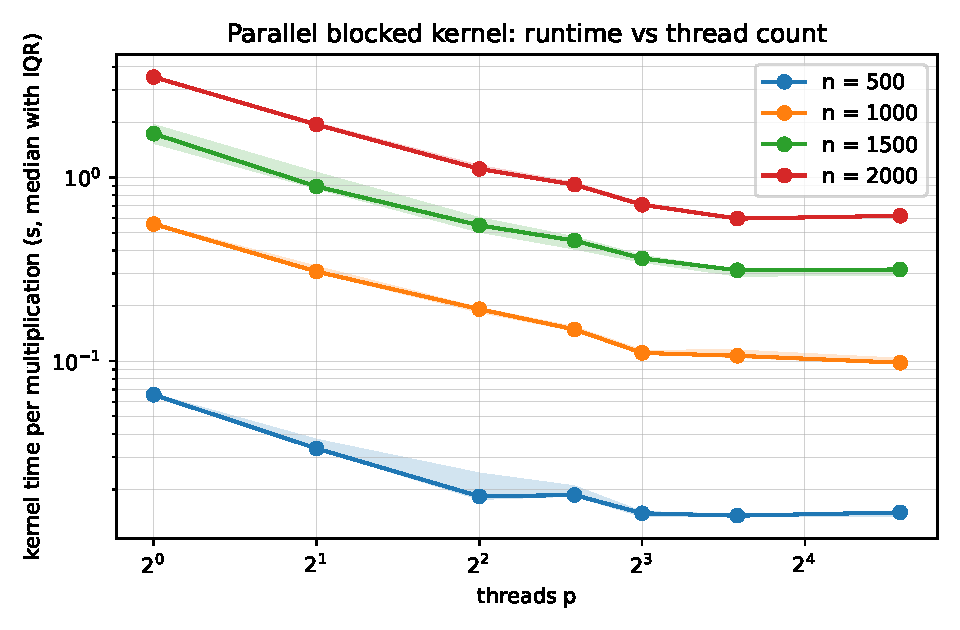
\includegraphics[width=\linewidth]{figures/median_time_vs_threads.pdf}
\caption{Kernel time per multiplication versus thread count (median with
IQR, log--log), per size.}
\label{fig:time}
\end{minipage}\hfill
\begin{minipage}[t]{0.49\linewidth}
\centering
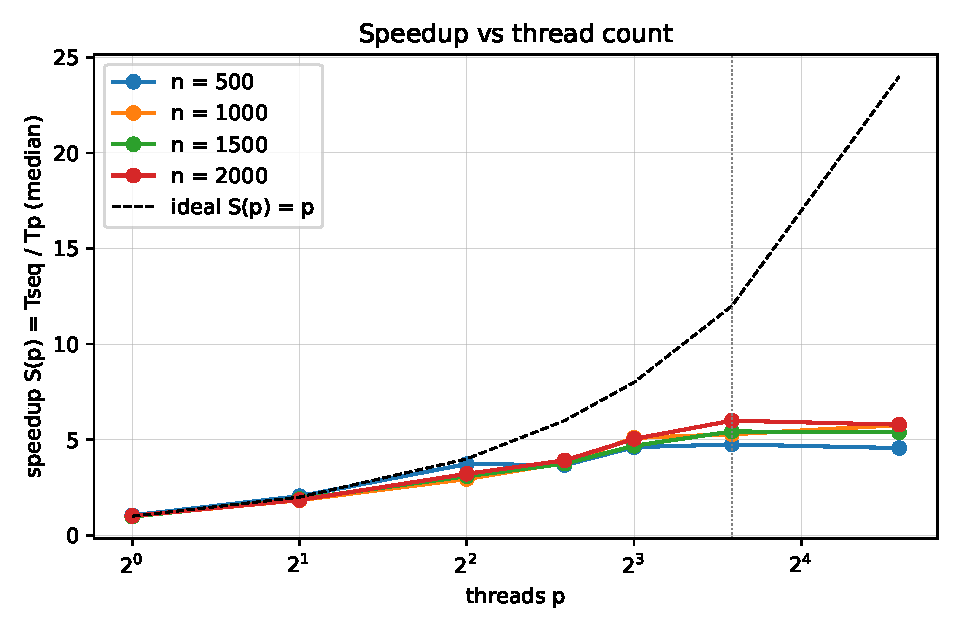
\includegraphics[width=\linewidth]{figures/speedup_vs_threads.pdf}
\caption{Speedup $S(p) = T_{\mathrm{seq}}/T_p$ versus thread count, per
size, against the ideal line $S(p) = p$.}
\label{fig:speedup}
\end{minipage}
\end{figure}

\subsection{Efficiency and the one-thread overhead}

Efficiency (Table~\ref{tab:speedup}, lower block;
Figure~\ref{fig:efficiency}) is near-ideal at $p = 2$ (0.92--1.02),
moderate at the physical-core count $p = 6$ (0.61--0.65), and drops below
0.5 once the hyper-threaded contexts are used ($p = 12$: 0.40--0.50) and
further under deliberate oversubscription ($p = 24$: 0.19--0.24, i.e.\
exactly about half of the $p = 12$ values, as expected when 24 runnable
threads time-share 12 hardware contexts). The parallel method with one
thread costs between $-4.2\%$ and $+1.9\%$ of the sequential baseline
(Figure~\ref{fig:overhead}): within the measurement noise of this
machine, so the dispatch and join of the pool are not what limits scaling
at these sizes.

\begin{table}[htbp]
\centering
\caption{Speedup $S(p) = T_{\mathrm{seq}}/T_p$ (upper block, from
medians) and efficiency $E(p) = S(p)/p$ (lower block) at each size and
thread count.}
\label{tab:speedup}
\begin{tabular}{rccccccc}
\toprule
$S(p)$ \textbackslash\ $p$ & 1 & 2 & 4 & 6 & 8 & 12 & 24 \\
\midrule
500  & 1.04 & 2.05 & 3.73 & 3.67 & 4.61 & 4.75 & 4.56 \\
1000 & 1.01 & 1.84 & 2.95 & 3.80 & 5.10 & 5.28 & 5.76 \\
1500 & 0.98 & 1.90 & 3.09 & 3.75 & 4.68 & 5.43 & 5.38 \\
2000 & 1.02 & 1.85 & 3.22 & 3.92 & 5.04 & 6.00 & 5.79 \\
\midrule
$E(p)$ \textbackslash\ $p$ & 1 & 2 & 4 & 6 & 8 & 12 & 24 \\
\midrule
500  & 1.04 & 1.02 & 0.93 & 0.61 & 0.58 & 0.40 & 0.19 \\
1000 & 1.01 & 0.92 & 0.74 & 0.63 & 0.64 & 0.44 & 0.24 \\
1500 & 0.98 & 0.95 & 0.77 & 0.63 & 0.59 & 0.45 & 0.22 \\
2000 & 1.02 & 0.92 & 0.80 & 0.65 & 0.63 & 0.50 & 0.24 \\
\bottomrule
\end{tabular}
\end{table}

\begin{figure}[htbp]
\centering
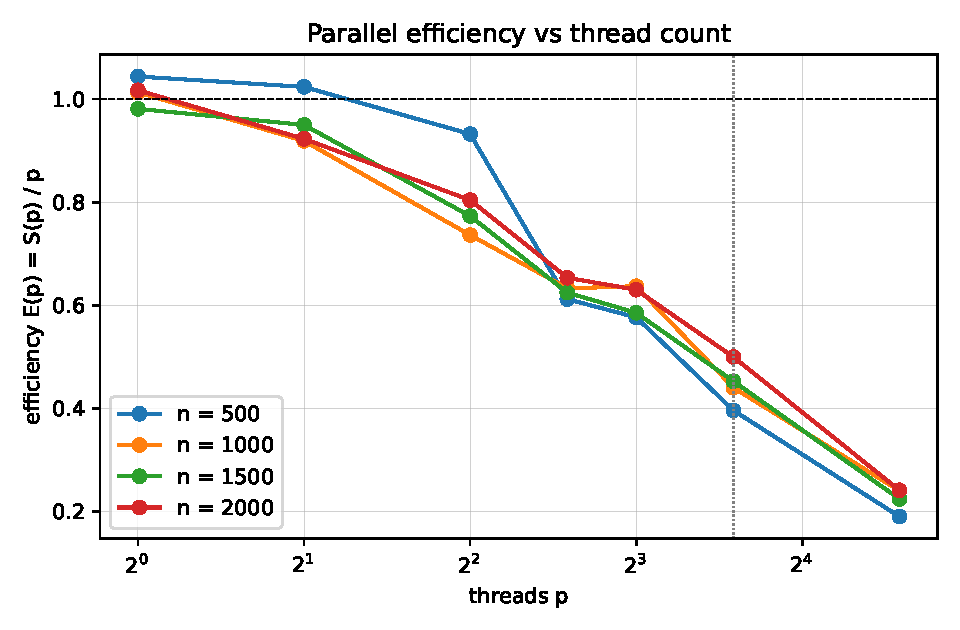
\includegraphics[width=\linewidth]{figures/efficiency_vs_threads.pdf}
\caption{Parallel efficiency $E(p) = S(p)/p$ versus thread count, per size;
the dashed line marks $E = 1$ (ideal) and the dotted vertical line the 12
logical processors.}
\label{fig:efficiency}
\end{figure}

\begin{figure}[htbp]
\centering
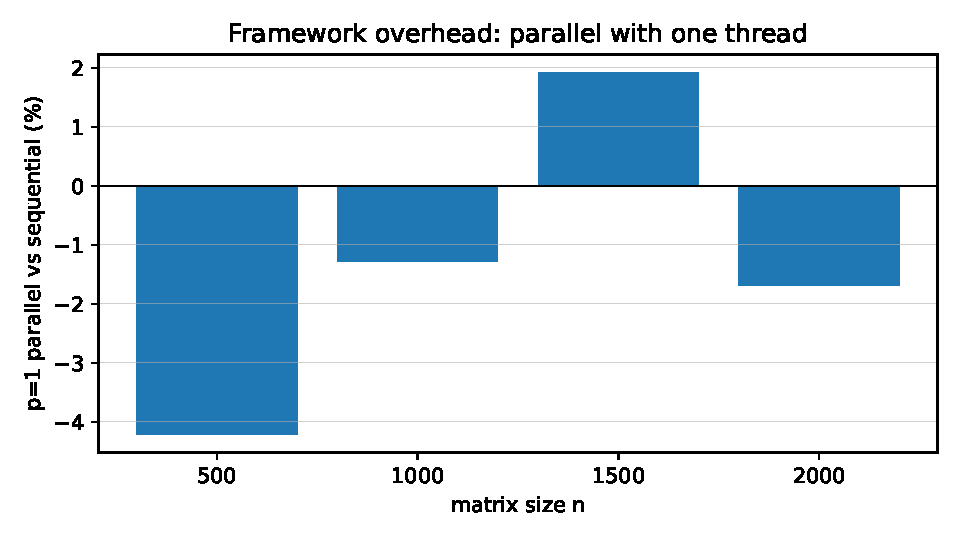
\includegraphics[width=\linewidth]{figures/framework_overhead.pdf}
\caption{Framework overhead: relative difference between the parallel
method with one thread and the sequential baseline, per size.}
\label{fig:overhead}
\end{figure}

\subsection{Memory}

Peak resident memory (Figure~\ref{fig:memory}) is dominated by the JVM
floor and the three dense matrices ($24n^2$ bytes: 57~MiB measured at
$n = 500$, 215~MiB at $n = 2000$ against 6~MB and 96~MB of theoretical
matrix storage). The thread count barely moves it: at $n = 2000$ the RSS
spans 215.9--217.2~MiB across all $p$ (0.6\% of range), because worker
stacks are small and mostly uncommitted at these depths. One excursion is
visible ($n = 1500$, $p = 24$: 159.9~MiB against about 141~MiB otherwise),
consistent with stack or JIT-commit behaviour under oversubscription
rather than with the matrix data, which is identical for every $p$.

\begin{figure}[htbp]
\centering
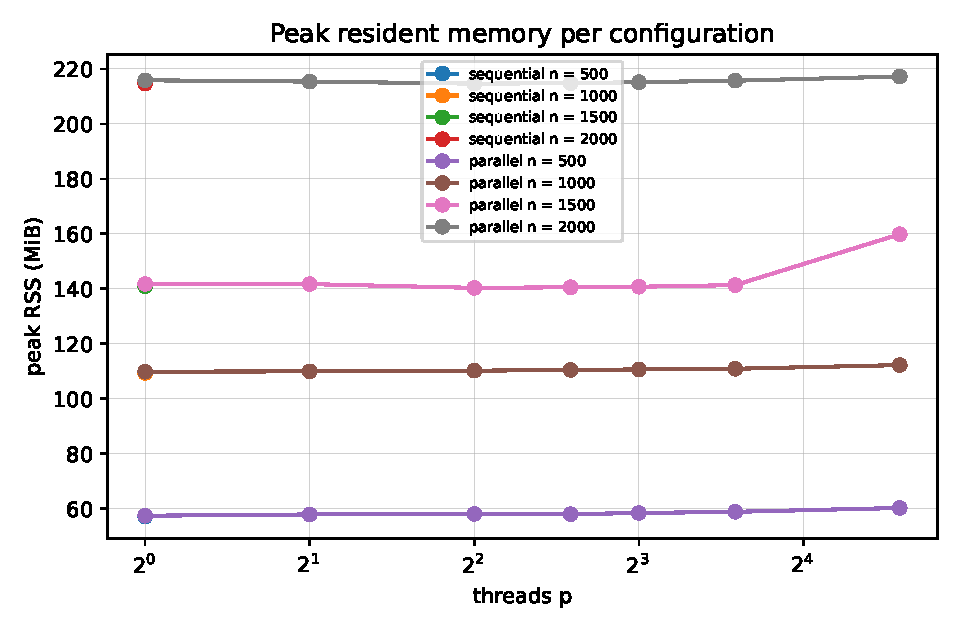
\includegraphics[width=\linewidth]{figures/peak_rss_vs_threads.pdf}
\caption{Peak resident memory versus thread count, per size and method.}
\label{fig:memory}
\end{figure}

\clearpage
\section{Discussion}
\label{sec:discussion}

\paragraph{When does parallel execution help?}
The evidence of Table~\ref{tab:speedup} and Figure~\ref{fig:speedup}
answers the research question with three regimes. First, parallelism pays
off at every tested size from $p = 2$ onwards, and the benefit grows with
$n$: at $p = 6$ (the physical cores) the speedup rises from 3.67
($n = 500$) to 3.92 ($n = 2000$), and the best cell of the whole campaign
is $S(12) = 6.00$ at $n = 2000$ --- per-multiplication overheads are
amortised over more work as $n$ grows, exactly as the
$T_p = T_{\mathrm{seq}}/p + T_{\mathrm{overhead}}$ model of
Section~\ref{sec:background} predicts. Second, the useful region ends at
the physical-core count: efficiency is 0.92--1.02 at $p = 2$ but only
0.61--0.65 at $p = 6$, and it falls below 0.5 once the hyper-threaded
contexts carry two workers each ($p = 12$: 0.40--0.50). The shared
execution units and the shared last-level cache, not the algorithm, set
this ceiling~\cite{hennessy2017}. Third, the deliberately oversubscribed
region ($p = 24$ on 12 hardware contexts) does not help: $E(24)$ is
0.19--0.24, about half of $E(12)$, and the median time is worse than at
$p = 12$ for $n = 1500$ (0.315 vs.\ 0.312~s) and $n = 2000$ (0.618 vs.\
0.596~s) while being marginally better for $n = 500$ and $n = 1000$
within noise. More threads than hardware contexts never reliably help;
they only add scheduling contention.

\paragraph{Framework overhead is not the bottleneck.}
With one thread the parallel method costs between $-4.2\%$ and $+1.9\%$
of the sequential baseline (Figure~\ref{fig:overhead}); the sign flips
because a $-4.2\%$ ``speedup'' at one thread cannot come from parallelism
and therefore measures machine noise (turbo/thermal state), not an
algorithmic effect. The dispatch and join of a prestarted pool are thus
inside the noise floor of this machine at these sizes, so the sub-linear
speedups observed beyond $p = 2$ must be attributed to hardware sharing
and to partitioning granularity, not to task-management cost. The
partitioning itself is near-perfect for large $n$: $n = 2000$ has
$\lceil 2000/64 \rceil = 32$ tiles, comfortably more than $p = 12$, so
tile ranges differ by at most one tile ($\le 3\%$ of the work).

\paragraph{Non-monotonicities and variability.}
Speedup is not monotone in $p$: for $n = 500$ it dips at $p = 6$ (3.67)
with respect to $p = 4$ (3.73), and for $n = 1000$ it jumps from 5.10 at
$p = 8$ to 5.76 at $p = 24$ after a plateau at $p = 12$. The raw samples
explain both without new physics: the $n = 500$ cells are extremely short
(14--19~ms) and noisy --- the $p = 4$ cell has a 38\% IQR --- so a few
fast or slow samples move the median by more than a whole thread step,
while for $n = 1000$ the $p = 24$ median (97.9~ms) sits against 106.9~ms
at $p = 12$, a 9\% gap that overlaps the tails of both sample sets.
Where cells are long and stable ($n = 2000$: 2.9\% IQR at $p = 12$) the
ordering is regular. No configuration shows a superlinear speedup
($S(p) > p$ nowhere), so no frequency-scaling or cache-residency
explanation is required~\cite{hill2008}. The sequential baseline itself
carries a 26\% IQR at $n = 1500$: its raw samples drift from 1949~ms to
1488~ms across the seven repetitions, the signature of thermal throttling
on a laptop during a multi-second single-threaded kernel. Every ratio
$S(p)$ divides by this drifting $T_{\mathrm{seq}}$, so the $n = 1500$
speedups inherit that uncertainty; medians were used throughout to limit
its effect.

\paragraph{Memory.}
Peak RSS is essentially independent of $p$ (0.6\% range at $n = 2000$),
which confirms that the parallel method's extra cost is thread stacks and
pool bookkeeping, not duplicated data: the partitioned design writes one
shared output and reads the same inputs from every thread. The single
159.9~MiB excursion at $n = 1500$, $p = 24$ is consistent with stack or
JIT code committed under oversubscription, and it is 19~MiB --- three
orders of magnitude below the ~1.5~GB ``small heaps'' that a naive
copy-per-thread design would need.

\subsection{Threats to validity}

Results are scoped to one machine, one JVM, one kernel (cache-blocked
$i$-$k$-$j$, tile 64, not tuned), the tested sizes ($n \le 2000$) and the
declared thread counts. The machine is a laptop: frequency scaling and
thermal behaviour affect the single-threaded baseline
($T_{\mathrm{seq}}$) and hence every ratio built on it. WSL2 adds a
virtualisation layer whose scheduling of the 12 logical processors is not
under the experimenter's control; the affinity mask was left at its
default (\texttt{0-11}) and recorded, not narrowed. Only one partitioning
strategy (contiguous $i$-tiles) and one runtime mechanism
(\texttt{ThreadPoolExecutor}) were tested.

\section{Conclusions}
\label{sec:conclusions}

\paragraph{Answers to the research question.}
(1) \emph{Parallel execution helps at every tested size, but only up to a
point}: the same kernel with $p$ threads reaches $6.00\times$ speedup
($n = 2000$, $p = 12$) and near-ideal efficiency at $p = 2$, while
efficiency at the physical-core count ($p = 6$) is already 0.61--0.65.
(2) \emph{Adding threads beyond the physical cores has sharply
diminishing returns, and oversubscription is never a reliable win}:
$E(12) \le 0.50$ and $E(24) \in [0.19, 0.24]$, with median times at
$p = 24$ worse than at $p = 12$ for the two largest sizes. (3) \emph{The
framework overhead of this design is not what limits scaling}: a single
thread stays within $-4.2\%$ to $+1.9\%$ of the sequential baseline, so
the sub-linear behaviour comes from hardware sharing and measurement
noise on a laptop, not from task dispatch. (4) \emph{The thread count is
irrelevant to memory}: peak RSS varies by 0.6\% across $p$ at $n = 2000$,
because the partitioned design shares all three matrices instead of
copying them per thread.

\paragraph{Recommendation.}
For this kernel on this class of machine, run the parallel method for
$n \ge 500$ with $p$ set to the number of \emph{physical} cores (6 here);
treat $p = 12$ as an opportunistic option for the largest sizes (it is
best or tied-best at $n = 1500$ and 2000) and never pay for $p = 24$.
Below $n = 500$ the multiplications are so short (tens of milliseconds)
that variability dominates and the sequential baseline is competitive;
there, batching or repeated multiplication is a better lever than more
threads. Re-measure $T_{\mathrm{seq}}$ on a thermally stable machine
before trusting fine-grained speedup differences, since the baseline
drifted by 26\% IQR at $n = 1500$ and every $S(p)$ divides by it.

\paragraph{What remains open.} Only one parallelisation strategy and one
mechanism were tested (work-stealing pools, row-cyclic partitioning and
parallel blocked variants with different tile sizes remain unexplored);
memory-bandwidth saturation was not measured directly (no hardware
counters); the vectorisation extension of the assignment was declared not
undertaken; and the largest tested size ($n = 2000$) is far below the
point where distributed execution (assignment 4) becomes necessary.

\clearpage
\section{References}
\swallownextsectionstar
\begin{thebibliography}{9}
    \bibitem{amdahl1967}
    G.~M. Amdahl, ``Validity of the single processor approach to achieving
    large scale computing capabilities,'' in \emph{Proc. AFIPS Spring Joint
    Computer Conference (SJCC)}, vol.~30, 1967, pp. 483--485.

    \bibitem{hill2008}
    M.~D. Hill and M.~R. Marty, ``Amdahl's law in the multicore era,''
    \emph{Computer}, vol.~41, no.~7, pp. 33--38, 2008.

    \bibitem{lam1991}
    M.~Lam, E.~E. Rothberg, and M.~D. Smith, ``The cache performance and
    optimizations of blocked algorithms,'' in \emph{Proc. 4th Int. Conf. on
    Architectural Support for Programming Languages and Operating Systems
    (ASPLOS)}, 1991, pp. 63--74.

    \bibitem{hennessy2017}
    J.~L. Hennessy and D.~A. Patterson, \emph{Computer Architecture: A
    Quantitative Approach}, 6th~ed. Morgan Kaufmann, 2017.

    \bibitem{lea2006}
    D.~Lea, \emph{Java Concurrency in Practice}. Addison-Wesley, 2006.
\end{thebibliography}

\section{Reproducibility materials}

All materials ship with this report: the Java (Maven) and Python sources;
the JUnit tests and the independent NumPy cross-check; the input
generator; the raw campaign CSVs
(\texttt{parallel\_}\allowbreak\texttt{time\_}\allowbreak\texttt{raw.csv},
\texttt{memory\_}\allowbreak\texttt{raw.csv} and \texttt{run\_log.txt});
and the figure script plus figure PDFs. They are attached as the archive
\texttt{Assignment03\_}\allowbreak\texttt{Lorenzo\_}\allowbreak
\texttt{Materials.zip} to the \texttt{assignment-03}
release of the course repository. From the project root, inside WSL2:

\begin{verbatim}
.venv/bin/python python/generate_inputs.py
mvn -q verify
mvn -q -DskipTests package
.venv/bin/python python/correctness_check.py
.venv/bin/python -m compileall python
.venv/bin/python python/run_experiments.py   # campaign
.venv/bin/python python/plot_results.py      # figures/*.pdf
\end{verbatim}

Exact toolchain versions and the full protocol are documented in
\texttt{README.md}. Runner exit codes: 0 (ok), 2 (invalid arguments), 3
(time budget exceeded), 4 (missing input files). The input binaries are
regenerated deterministically from seed 42 and are not shipped.
\url{https://github.com/aythamilorenzo/bigdata-individual-assignments}.\footnote{Generative AI
tools were utilized solely to refine the stylistic quality, grammar, and
technical phrasing of this report.}

\end{document}
